%
% File eacl2009.tex
%
% Contact  oflazer@gmail.com or das@ling.uni-potsdam.de
%%

%% Based on the style files for EACL 2006 by 
%%e.agirre@ehu.es or Sergi.Balari@uab.es
%% and that of ACL 08 by Joakim Nivre and Noah Smith

\documentclass[11pt]{article}
\usepackage{eacl2009}
\usepackage{times}
\usepackage{url}
\usepackage{latexsym}
\usepackage[icelandic]{babel}
\usepackage[T1]{fontenc}
\usepackage[utf8]{inputenc}
\usepackage{graphicx}
\usepackage{wrapfig}

\setlength\titlebox{9.5cm}    % You can expand the title box if you
% really have to

\title{Rýnir - Tækniskýrsla}

\author{Arnór Barkarson\\
  Reykjavík University\\
  Reykjavík, Iceland\\
  {\tt arnorbarkar@ru.is}  \And  
  Ragnar Lárus Sigurðsson\\
  Reykjavík University\\
  Reykjavík, Iceland\\
  {\tt  ragnarls08@ru.is}\\ \And 
  Þórður Arnarsson\\
  Reykjavík University\\
  Reykjavík, Iceland\\
  {\tt  thordura08@ru.is}  \And 
  Gunnar Sveinsson\\
  Reykjavík University\\
  Reykjavík, Iceland\\
  {\tt  gunnarsve06@ru.is} 
}



\date{}

\begin{document}
\maketitle


\section{Summary}
\section{Introduction}
\section{Body}
\subsection{Fourier transformations}
Fourier transformations eru stærðfræðilegar aðgerðir sem brjóta merki niður í tíðnir þess. Slíkt gátum við nýtt okkur með því að láta umbreyta 
tímalínu í tíðnir. Ef áberandi tíðni fannst þá er endurtekning í tímalínunni. Sem dæmi um slíkt í okkar kerfi er þegar 
rafmagnsnotkun í ótilgreindu landi er skoðuð.\\

\begin{wrapfigure}{l}{6cm}
%\begin{figure}
 \begin{center}
 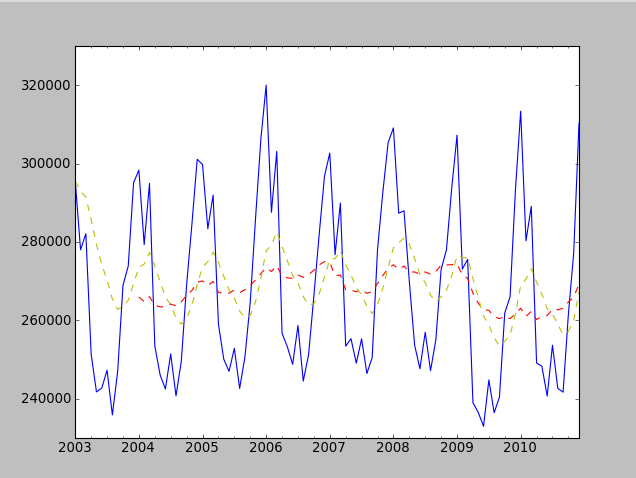
\includegraphics[width=.45\textwidth]{Rafmagnsnotkun.png}
 \caption{Tímalína um rafmagnsnotkun}
  \end{center}
%\end{figure}
\end{wrapfigure}
\hfill
\\\\\\\\\\\\\\\\\\\\\\\\\\\\\\\\\\\

Það má sjá að tímalínan hefur ákveðnar endurtekningar, nánar til tekið þá er mikil notkun á veturna en lítil á sumrin.
Þessa föstu sveiflu í tímalinunni greinir Fourier og skilar eftirfarandi grafi. 
Það segir okkur að á 12 staka fresti í tímalínunni er endurtekning.

\begin{wrapfigure}{l}{6cm}
%\begin{figure}
 \begin{center}
 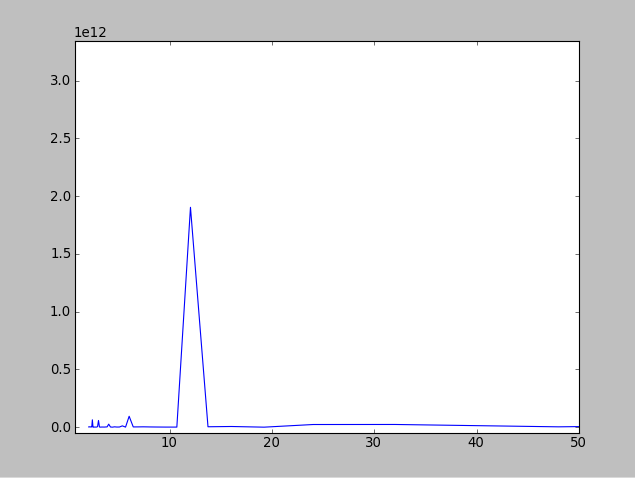
\includegraphics[width=.45\textwidth]{Fourier.png}
 \caption{Fourier um rafmagnsnotkun}
  \end{center}
%\end{figure}
\end{wrapfigure}
\hfill
\\\\\\\\\\\\\\\\\\\\\\\\\\\\\\\\\\\

\subsection{Hlaupandi meðaltal (HM)}
Í tölfræði er hlaupandi meðaltal, einnig kallað fljótandi meðaltal, notað til greiningar á gagnamengi. 
Er það gert með því að mynda röð meðaltala úr mismunandi hlutmengjum heildarmengisins.\\
Ef gefin er röð $K$ talna og ákveðin stærð ramma (hlutmengis) er $N$, þá er fljótandi meðaltal fundið með því að fyrst reikna meðaltal 
talna úr sæti $0,1,\dots,N-1$. Þá er ramminn færður fram um eitt sæti og meðaltal fundið af tölum í sætum $1,2,\dots,N$. 
Þessi aðgerðarröð er endurtekin yfir alla talnaröðina, $K-N$ sinnum.  \\
$HM = \frac{x+(x+1)+\dots+(x+(N-1))}{N}$
\\
Línan sem tengir svo saman öll meðaltölin er hið fljótandi meðaltal þar sem hver punktur á línunni samsvarar 
meðaltali viðkomandi hlutmengis í heildarmengi ganganna sem verið er að meta. 
 
\subsection{Vegið hlaupandi meðaltal (VHM)}
Hlaupandi meðaltal getur einnig notað ójöfn gildi fyrir hvert stak á línunni.
Þá er um vegið meðaltal að ræða og er meðaltalinu gefin einhver margfeldisáhrif eftir því hvar á línunni það er staðsett. 
Það vægi breytist línulega. Summu margfeldi allra gildana í tilteknum ramma er svo deilt með summu allra mergfeldanna. 
Ef um ramma af stærð 10 er að ræða og gildin eru margfölduð eftir sætisröð, þá fæst: \\
$VHM = \frac{x+2(x+1)+3(x+2)+\dots+(x+10(N-1))}{1+2+\dots+10}$


\subsection{Bollinger bands}
\label{sec:third}

Bollinger bönd eru upprunalega þróuð sem greiningartól á þróun verðbréfaverða. 
Tilgangur þess er að veita viðeigandi skilgreiningu hágum og lágum gildum. Einnig hefur þessari aðferð verið beitt á ýmis önnur
vandamál með misgóðum niðurstöðum. \\

Bollinger bönd samanstanda af
\begin{itemize}
  \item Miðband, $N-lotu$ einfalt hlaupandi meðaltal.
  \item Efra band, $N-lotu$ staðalfrávik margfaldað með $K$, fyrir ofan miðbandið ($HM + K\sigma$).
  \item Neðra band, $N-lotu$ staðalfrávik margfaldað með $K$, fyrir neðan miðbandið ($HM - K\sigma$).
\end{itemize}
Bollinger bönd nýtast því vel til greininga hvar í tímalínu óeðlileg hækkun eða lækkun á sér stað.
\subsubsection{Okkar útfærsla á Bollinger}
...
Útfærslan okkar byggist á því að keyra ítranir af Bollinger böndum á tímalínu með mismunandi gluggastærð, 
þar sem gluggastærðin er að hluta til ákvörðuð af stærð tímalínunnar. 
Hverri ítrun er síðan gefið ákveðið vægi miðað við gluggastærð hennar, væginu er hagað þannig að 100\% vægi skiptist niður á ítranirnar.
...

\begin{picture}(2,2)
  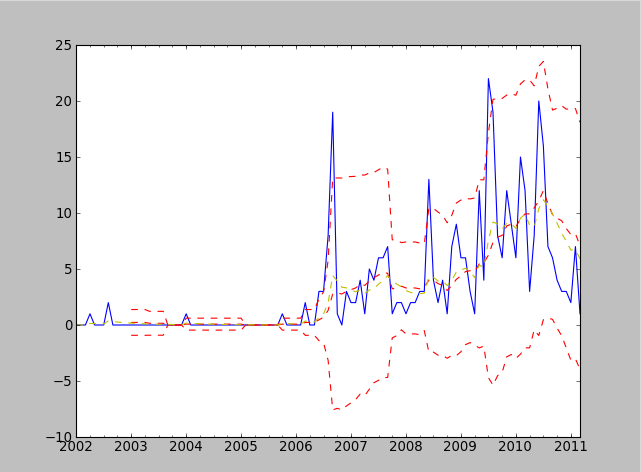
\includegraphics[width=.45\textwidth]{bollinger.png}
  %\caption{Bollinger bands\label{fig:first}}
\end{picture}




\section{Conclusion}
\section{Abstract}

 



\end{document}
